%%%% SIMULATION FRAMEWORK %%%%
\chapter{Simulation framework for performance characterization}\label{chap:06_Simulation_Framework}
In this chapter, we lay out a simulation framework for characterizing the performance of different navigational techniques.
In the following sections, we describe the geometry of the simulated sound field, define the parameters of the simulations, and enumerate the metrics which will be computed.
In each of the following chapters, we present results characterizing and comparing different navigational methods obtained by conducting the simulations described here.
Additionally, in \chapref{chap:10_Experimental_Validation}, an experimental validation of the simulations is presented.

\section{Microphone and source geometries}\label{sec:06_Simulation_Framework:Geometry}
In this section we present the ambisonics microphone array geometries used in the subsequent numerical simulations.
In both cases described below, the listener traverses a straight line away from the microphone(s), which will allow us to explore any dependence on source azimuth relative to the direction of travel (see \secref{sec:06_Simulation_Framework:Azimuth_Dependence}).

\subsection{Single-microphone array}\label{sec:06_Simulation_Framework:Point_Geometry}
Consider a single-microphone array geometry, illustrated in \figref{fig:06_Simulation_Framework:Point_Geometry}, in which a single ambisonics microphone ($P = 1$) is separated from the origin by a distance $u$ and placed along the longitudinal $x$-axis, such that its position is given by $\vec{u}_1 = (u,0,0)$.
(Recall that, according to our coordinate system described in \secref{sec:02_Acoustical_Theory:Coordinate_System}, the $+x$-axis points forward from the listener, the $+y$-axis points to the left, and the azimuth $\phi$ measures the angle away from straight ahead.)
In this configuration, we define the \textit{navigable region} as the segment of the $x$-axis connecting the origin and microphone position, i.e., all listener positions $\vec{r}_0 = (x_0, 0, 0)$ where $x_0 \in [0,u]$.

% Diagram of source/mic positions
\begin{figure}[t]
\centering
  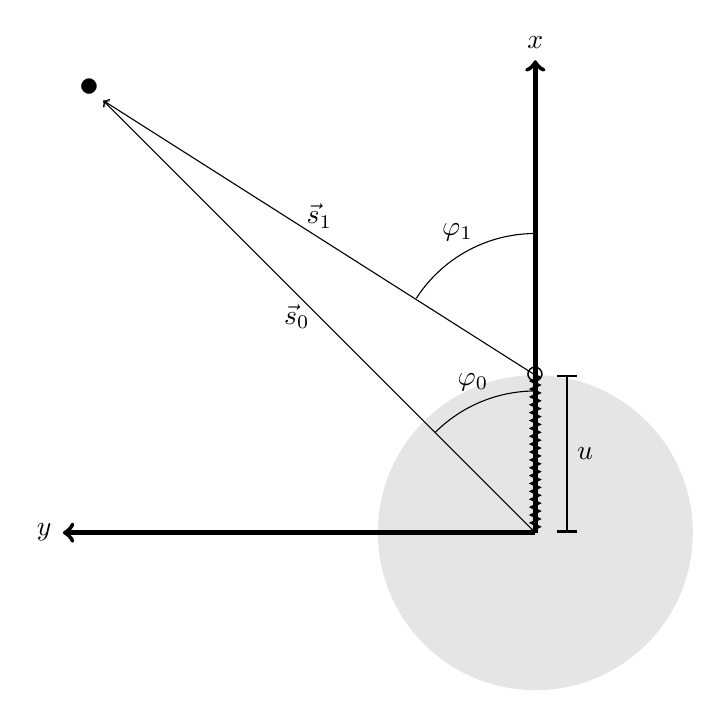
\begin{tikzpicture}[scale=4]
% Parameters
\def\radius{1.5};
\def\arrowScale{0.97};

\def\micSpacing{1};
\def\micL{-0.5*\micSpacing};

\def\sourceRadius{2};
\def\sourceAzimuth{45}
\pgfmathsetmacro\sourceY{cos(-\sourceAzimuth)*\sourceRadius}
\pgfmathsetmacro\sourceX{sin(-\sourceAzimuth)*\sourceRadius}

\pgfmathsetmacro\sourceLAzimuth{-atan(\sourceX/(\sourceY+\micL))}

\def\arcRadius{0.45};
\pgfmathsetmacro\arcY{cos(-\sourceAzimuth/2)*\arcRadius}
\pgfmathsetmacro\arcX{sin(-\sourceAzimuth/2)*\arcRadius}
\pgfmathsetmacro\arcLY{cos(-\sourceLAzimuth/2)*\arcRadius}
\pgfmathsetmacro\arcLX{sin(-\sourceLAzimuth/2)*\arcRadius}

% Coordinate system
\draw[ultra thick,->] (0,0) -- (0,\radius) node[above]{$x$};
\draw[ultra thick,->] (0,0) -- (-\radius,0) node[left]{$y$};

% Arrows
\node at (\sourceX,\sourceY){\Large $\bullet$}; % source
\draw[->] (0,0) -- (\arrowScale*\sourceX,\arrowScale*\sourceY) node[left, pos=0.5]{$\vec{s}_0$}; % origin
\draw[->] (0,-\micL) -- (\arrowScale*\sourceX,\arrowScale*\sourceY) node[above, pos=0.5]{$\vec{s}_1$}; % mic
\draw[thick, decoration = {zigzag, segment length = 1mm, amplitude = 0.5mm}, decorate] (0,0) -- (0,-\micL); % navigable region

% Arcs
\draw[domain=90:(90+\sourceAzimuth)] plot ({\arcRadius*cos(\x)}, {\arcRadius*sin(\x)});
\node at (1.15*\arcX,1.15*\arcY){$\varphi_0$};

%\draw[dashed,->] (\micL,0) -- (\micL,\arcRadius); % left mic
\draw[domain=90:(90+\sourceLAzimuth)] plot ({\arcRadius*cos(\x)}, {\arcRadius*sin(\x) - \micL});
\node at (1.15*\arcLX,1.15*\arcLY - \micL){$\varphi_1$};

% Mic positions
\node at (0,-\micL){\Large $\circ$};
\draw[thick,|-|] (0.1,0) -- (0.1,-\micL) node[right, pos=0.5]{$u$};

\fill [color=black,opacity=0.1] (0,0) circle (\micSpacing/2);

\end{tikzpicture}
  \caption[Diagram of the array geometry for extrapolation simulations.]{
  Diagram of a microphone (empty circle) and a single source (filled circle).
  The shaded gray disk indicates the interior region, where $r < u$.
  The jagged line segment indicates the navigable region, where $x \in [0,u]$ and $y = z = 0$.}
  \label{fig:06_Simulation_Framework:Point_Geometry}
\end{figure}

A single point source is placed on the horizontal plane at $\vec{s}_0 = (s_0 \cos \varphi_0, s_0 \sin \varphi_0, 0)$.
From the position of the microphone, the apparent source position is given by
$\vec{s}_1 = \vec{s}_0 - \vec{u} = (s_1 \cos \varphi_1, s_1 \sin \varphi_1, 0)$,
such that the apparent source azimuth is $\varphi_1$ and the relative source distance from the microphone is $s_1$.

We further define a nondimensional geometrical parameter $\gamma = r / u$.
Here we refer to the region with $\gamma > 1$ as the \textit{exterior region} and that with $\gamma < 1$ as the \textit{interior region} (see \figref{fig:06_Simulation_Framework:Point_Geometry}).

\subsection{Linear microphone array}\label{sec:06_Simulation_Framework:Linear_Geometry}
Consider a linear microphone array geometry, illustrated in \figref{fig:06_Simulation_Framework:Linear_Geometry}, in which a pair of ambisonics microphones ($P = 2$) are separated by a distance $\Delta = 2u$, equidistant from the origin and placed along the lateral $y$-axis, such that their positions are given by $\vec{u}_1 = (0,\Delta/2,0)$ and $\vec{u}_2 = (0,-\Delta/2,0)$.
In this configuration, we define the \textit{navigable region} as the segment of the $y$-axis connecting the two microphone positions, i.e., all listener positions $\vec{r}_0 = (0, y_0, 0)$ where $y_0 \in [-\Delta/2,\Delta/2]$.
Here also we define the same nondimensional geometrical parameter, now given by $\gamma = r / (\Delta / 2) = r / u$.

% Diagram of source/mic positions
\begin{figure}[t]
\centering
  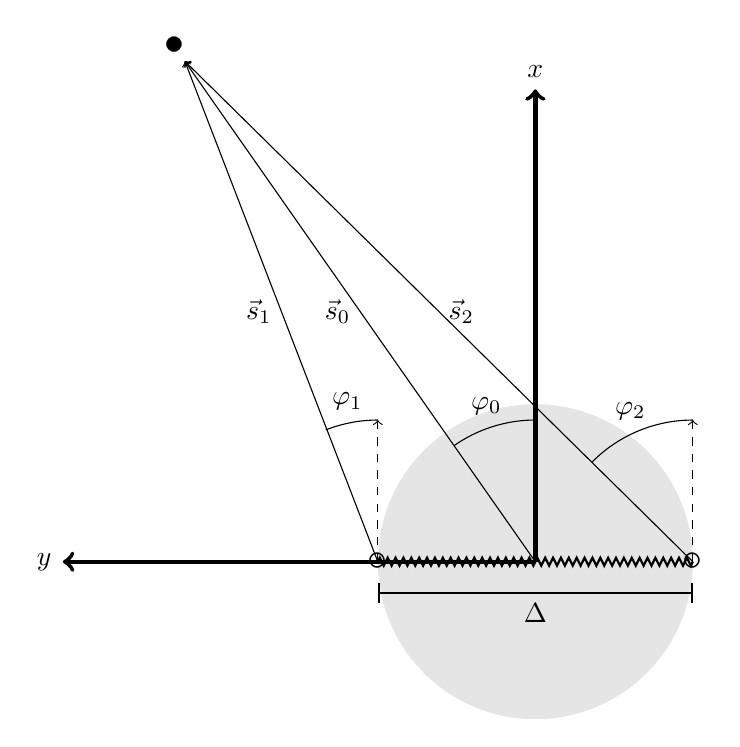
\begin{tikzpicture}[scale=4]
% Parameters
\def\radius{1.5};
\def\arrowScale{0.97};

\def\micSpacing{1};
\def\micL{-0.5*\micSpacing};
\def\micR{0.5*\micSpacing};

\def\sourceRadius{2};
\def\sourceAzimuth{35}
\pgfmathsetmacro\sourceY{cos(-\sourceAzimuth)*\sourceRadius}
\pgfmathsetmacro\sourceX{sin(-\sourceAzimuth)*\sourceRadius}

\pgfmathsetmacro\sourceLAzimuth{-atan((\sourceX-\micL)/\sourceY)}
\pgfmathsetmacro\sourceRAzimuth{-atan((\sourceX-\micR)/\sourceY)}

\def\arcRadius{0.45};
\pgfmathsetmacro\arcY{cos(-\sourceAzimuth/2)*\arcRadius}
\pgfmathsetmacro\arcX{sin(-\sourceAzimuth/2)*\arcRadius}
\pgfmathsetmacro\arcLY{cos(-\sourceLAzimuth/2)*\arcRadius}
\pgfmathsetmacro\arcLX{sin(-\sourceLAzimuth/2)*\arcRadius}
\pgfmathsetmacro\arcRY{cos(-\sourceRAzimuth/2)*\arcRadius}
\pgfmathsetmacro\arcRX{sin(-\sourceRAzimuth/2)*\arcRadius}

% Coordinate system
\draw[ultra thick,->] (0,0) -- (0,\radius) node[above]{$x$};
\draw[ultra thick,->] (0,0) -- (-\radius,0) node[left]{$y$};

% Arrows
\node at (\sourceX,\sourceY){\Large $\bullet$}; % source
\draw[->] (0,0) -- (\arrowScale*\sourceX,\arrowScale*\sourceY) node[left, pos=0.5]{$\vec{s}_0$}; % origin
\draw[->] (\micL,0) -- (\arrowScale*\sourceX,\arrowScale*\sourceY) node[left, pos=0.5]{$\vec{s}_1$}; % left mic
\draw[->] (\micR,0) -- (\arrowScale*\sourceX,\arrowScale*\sourceY) node[right, pos=0.5]{$\vec{s}_2$}; % right mic
\draw[thick, decoration = {zigzag, segment length = 1mm, amplitude = 0.5mm}, decorate] (\micL,0) -- (\micR,0); % navigable region

% Arcs
\draw[domain=90:(90+\sourceAzimuth)] plot ({\arcRadius*cos(\x)}, {\arcRadius*sin(\x)});
\node at (1.15*\arcX,1.15*\arcY){$\varphi_0$};

\draw[dashed,->] (\micL,0) -- (\micL,\arcRadius); % left mic
\draw[domain=90:(90+\sourceLAzimuth)] plot ({\arcRadius*cos(\x) + \micL}, {\arcRadius*sin(\x)});
\node at (1.15*\arcLX + \micL,1.15*\arcLY){$\varphi_1$};

\draw[dashed,->] (\micR,0) -- (\micR,\arcRadius); % right mic
\draw[domain=90:(90+\sourceRAzimuth)] plot ({\arcRadius*cos(\x) + \micR}, {\arcRadius*sin(\x)});
\node at (1.15*\arcRX + \micR,1.15*\arcRY){$\varphi_2$};

% Mic positions
\node at (\micL,0){\Large $\circ$};
\node at (\micR,0){\Large $\circ$};
\draw[thick,|-|] (\micL,-0.1) -- (\micR,-0.1) node[below, pos=0.5]{$\Delta$};

\fill [color=black,opacity=0.1] (0,0) circle (\micSpacing/2);

\end{tikzpicture}
  \caption[Diagram of the array geometry for interpolation simulations.]{
  Diagram of a two-microphone array (empty circles) with a single source (filled circle).
  The shaded gray disk indicates the interior region, where $r < \Delta / 2$.
  The jagged line segment indicates the navigable region, where $y \in [-\Delta/2,\Delta/2]$ and $x = z = 0$.}
  \label{fig:06_Simulation_Framework:Linear_Geometry}
\end{figure}

Similar to the single-microphone case, the apparent source position from the position of the $p^\textrm{th}$ microphone is given by
$\vec{s}_p = \vec{s}_0 - \vec{u}_p = (s_p \cos \varphi_p, s_p \sin \varphi_p, 0)$,
such that the apparent source azimuth is $\varphi_p$ and the relative source distance from that microphone is $s_p$.

\section{Simulation parameters}\label{sec:06_Simulation_Framework:Parameters}
For extrapolation methods, we simulate recording of the sound field depicted in \figref{fig:06_Simulation_Framework:Point_Geometry} for a range of microphone positions, $u \in [0.1, 10]$~m, and all source positions $s_0 = \gamma u$ for $\gamma \in [0.1, 10]$.
In each simulation, we vary the source azimuth from $\varphi_0 = 0^\circ$ to $180^\circ$ in increments of $5^\circ$ and generate an artificial ambisonics impulse response at the microphone.
We then estimate, using each extrapolation method, the ambisonics impulse responses at translated listener positions from $x_0 = 0$ to $u$, taken in 20 equal increments.

For interpolation methods, we simulate recording of the sound field depicted in \figref{fig:06_Simulation_Framework:Linear_Geometry} for a range of microphone spacings, $\Delta \in [0.1, 10]$~m, and all source positions $s_0 = \gamma \Delta / 2$ for $\gamma \in [0.1, 10]$.
For those methods that require interpolation weights, we choose linear interpolation weights for each intermediate position between the microphones.
In each simulation, we vary the source azimuth from $\varphi_0 = 0^\circ$ to $90^\circ$ in increments of $5^\circ$ and generate an artificial ambisonics impulse response at each microphone.
We then estimate, using each interpolation method, the ambisonics impulse responses at intermediate listener positions from $y_0 = -\Delta/2$ to $\Delta/2$, taken in 20 equal increments.

In all simulations, unless stated otherwise, we choose $L_\textrm{in} = 4$ and $L_\textrm{out} = 1$.%
\footnote{Note that, for the metrics listed in \secref{sec:06_Simulation_Framework:Metrics}, only the localization model (described in \secref{sec:05_Proposed_Models:Localization_Model}) depends on $L_\textrm{out}$; all of the other metrics, by construction, use only the zeroth and first order signals.}
The sampling rate is 48~kHz and all impulse responses are calculated with 16,384~samples ($\approx 341$~ms).
Additionally, unless stated otherwise, we filter all point-source ambisonics impulse responses with the near-field compensation high-pass filters given in \eqnref{eq:02_Acoustical_Theory:NearField_HPF}, with order-dependent corner frequencies equal to $f_l = (200 \times l)$~Hz.

\subsection{Source azimuth dependence}\label{sec:06_Simulation_Framework:Azimuth_Dependence}
In order to explore the basic properties of a given navigational method, we consider a representative far-field scenario and compute the effective frequency response induced by translation.
For these simulations, we pick $s_0 = 2.5$~m and $\gamma = 10$ (so $u = 0.25$~m for extrapolation methods and $\Delta = 0.5$~m for interpolation methods) and translate to $\vec{r}_0 = (0, 0, 0)$.
Then, for each source azimuth, we compute the induced frequency response, which is given by the ratio of the zeroth-order translated ambisonics signal, $A_0(k)$, to the zeroth-order reference ambisonics signal, $B_0(k)$, that would have been measured at $\vec{r}_0$.

\section{Metrics}\label{sec:06_Simulation_Framework:Metrics}
We ultimately compute errors incurred through navigation by each method using the following metrics:
\begin{enumerate}
\item the level error, $e_\lambda$, of the mean audible energy (MAE), as given in \secref{sec:04_Auditory_Models:Audible_Energy},
\item the spectral range, $\rho_\eta$, of the auditory band spectral error (ABSE), as given in \secref{sec:04_Auditory_Models:Coloration_Metrics:ABSE},
\item the localization error, $e_\nu$, as given in \eqnref{eq:04_Auditory_Models:Localization_Error}, for the localization vector model proposed in \secref{sec:05_Proposed_Models:Localization_Model}, and
\item the error, $e_\Psi$, in the diffuseness parameter, as given in \secref{sec:04_Auditory_Models:Diffuseness_Parameter}.
\end{enumerate}
In the following chapters, we plot these predicted errors, averaged over the entire navigable region (as defined above) and all source azimuths,%
\footnote{Note that doing so yields an effective navigable region which is disk-shaped relative to a single fixed source position and, due to symmetry, we need only compute these errors on half of the disk.}
for various combinations of source distance $s_0$ and either microphone distance $u$ (for extrapolation methods) or microphone spacing $\Delta$ (interpolation methods).